\chapter{Database Modeling}
\label{chap:database_modeling}

Modeling is a crucial phase of database design process.
Developing a database is just like building a house. 
Every one will agree that no construction work can go without solid design and documentation. 
It would sound a bit strange to hire construction workers straight ahead and tell them that we need a house that has 5 rooms, some toilets and expect a good result. Most probably some building would be produced, but we will agree that expectations and requirements of the later inhabitant could not be met properly.
Surely there are good reasons why the usual steps are followed strictly.
Let us move on from the analogy to the database domain. \\
When deploying a database from a scratch we may think of two short term advantages. Firstly, the time needed to have data stored somewhere would be much shorter and secondly the initial cost of the system could be lower. \\
But over time both of the advantages will most likely, if the database is not ridiculously small, get outnumbered by problems that will begin to appear. Maintenance of a poorly designed system (or not designed at all) is expansive and leads to numerous outages.\\

There are good reasons to why modeling has its place in a database development process:

\TODO{even shorter}
\begin{itemize}
	\item Higher quality.\\ Modeling push to thorough definition of the modeled problem. Once we know what to solve and what is the scope, it is much easier to come with different solutions and justify which of the proposed approaches is the most suitable one.
	
	\item Costs reduction.\\ Errors are identified thus can be caught in early stages, when they are easy to fix.
	
	\item Better documentation.\\ Data models form a nice piece of it, they are understandable by each of the involved stakeholders. When someone tries to understand the system, he can choose a data model on an appropriate level of abstraction that will introduce him the important aspects of the problem that suits his knowledge and qualification.
	
	\item Correctness.\\ Tracking whether high-level concepts were implemented and represented correctly in the end is made straightforward.
	
	\item Determining of consistency of the system.
	
	\item Deeper understanding.\\ During the design process we may learn a lot about properties of the data that we need or have and will be stored. These information are crucial for choosing an appropriate type of database, whether to stick with a relational database if so which DBMS is the one for us, or to look for a non-relational one.
\end{itemize}

\section{Data Model Perspectives}

\subsubsection{Vertical Division}

American National Standards Institute \cite{ANSIArchitecture75} came with a database structure called Three-schema architecture. It is formed by:
\begin{itemize}
	\item External Level \\ Database as a user sees it, view of the conceptual level. 
	\item Conceptual Level \\ Point of view of the enterprise that the database belongs to.
	\item Physical Level \\ The actual implementation.
\end{itemize}

The idea behind the structure was to create three different views that are independent of each other. 
For example change of the implementation that is tied with physical level would not affect any of the remaining levels if the structures remained the same. 
The important aspect is that this structure is used to describe finished product, it does not say anything about the design process that leads to the product and should not be mistaken with the data model structure proposed earlier \ref{DataModelsByAbstraction}.\\

On the other hand, to standardize process of designing a database Peter Chen\cite{Chen76theentity-relationship} identified four levels of view of data, where each of the levels has its important place: \\
\begin{enumerate}
	\item Information concerning entities and relationships which exist in our minds.
	\item Information structure-organization of information in which entities and relationships are represented by data.
	\item Access-path-independent\footnote{An \definition{access path} is a description how records stored in a database are retrieved by database management system\cite{AccessPathDefiniton}. The important part is that the path is specific for a DBMS technology.} data structure-the data structures which are not involved with search schemes, indexing schemes, etc.
	\item Access-path-dependent data structure.
\end{enumerate}

The categorization of data models have undergone some modifications, for example the first level is today omitted, to the one that is recognized nowadays. The differentiation takes takes into account  what is the audience that will work with a data model, whether it is someone who knows all about databases or a business person without technical background. The levels of abstraction used today\cite{SilberschatzKorthSudarshan10} are the following: 
\begin{itemize}
	\item Conceptual Data Models (High-Level) \\
	Reproduces real world objects along with their relationships and should be close to how business end-users perceive them.
	
	\item Logical Data Models (Implementation, Representational) \\
	In the middle between the two other model types there are representational data models which on the one hand are comprehensible by end-users and on the other hand are not too abstract so that they can be used as documentation for an actual database implementation of the modeled data.
	
	\item Physical Level Data Models(Low-Level) \\
	In contrast to conceptual models the physical ones are tied with how data are stored physically at storage media showing all specific internal details that may be overwhelming in the case that the reader is a computer specialist.
\end{itemize}


\subsubsection{Horizontal Division}

\subsubsection{Relational Data Model}

\TODO{Move to database section}
In the early days when navigational databases were trending, concretely hierarchical and network database, each of them was represented by corresponding data model. 
The key concept behind these databases was that records stored in databases should be found by navigating through link between objects. 
There were some issues about it. The biggest problem was that application code was too dependent on how data were actually placed physically and changes in data structures had influence on code that queried the storage had to be rewritten.
The advantage of navigational databases was their performance as following a link is much simpler operation than a join that is used instead in relational databases so they were considered better in terms of performance. Although, the efficiency was at price of inflexibility when reorganization of the storage was needed. Some solutions to this issue were proposed but they tended to worsen the performance.\\

As in this work we are dealing only with relational databases, for which relational data model is the foundation.
In 1969 Edgar F. Codd \cite{Codd69} brought the idea of relational database organization and the relational data model was born. \TODO{already described}

\subsubsection{Entity-Relationship Data Model}

The \definition{entity-relationship (ER) data model} was the direct answer for the four level architecture\cite{Chen76theentity-relationship} that covers the highest two levels and may be a basis for unified view of data. \\
It was an opposition to the three major data models that were used - relational, network and entity set model. His aim was to bring a data model that would reflect real-world objects and relations between them naturally, while having advantages of all the three already existing models. The mission seems to be successful as years have proven the ER data model to be the most suitable one for conceptual data modeling. Moreover, ER data models are used most commonly in logical data modeling as well.

\subsubsection{Enhanced-Entity-Relationship Data Model}

An extended version of ER data model was introduced later - \definition{enhanced-entity-relationship (EER) data model}. The main change is that concept sub-classes and super-classes, known as inheritance or is-a relationship, between entities was brought. \\ 

\TODO{conclusion}
Conceptual and logical data models are usually represented by ER data models. 
The question is what specific data model type is used for physical models. 
As the most low-level model type is tied directly with how a database is organized, physical models must obey the structure of database.

\subsection{Conceptual Data Model}

The purpose of a conceptual data model is to project to the model real-world and business concepts or objects. \\

\subsubsection{Characteristics}
\begin{itemize}
	\item Aimed to be readable and understandable by everyone.
	\item Is completely independent of technicalities like a software used to manage the data, DBMS, data types etc.
	\item Is not normalized.
\end{itemize}

A real world object is captured by an \definition{entity} in conceptual model. \\
For further description of objects that we are interested in \definition{attributes} are used, those are properties of entities. Only the important ones are listed. \footnote{Definitions varies and in some literature can be even found that a conceptual entity lacks attributes. We assume that the entity can contain important attributes as it is more common interpretation and modeling tools have attributes support on conceptual layer as well.} \\
Also \definition{relationships} between objects are necessary to provide full view of the section of the world that a data model resembles. \\

To illustrate it on an example, if our modeling domain is education, then an entity may be a teacher or lesson. 
A lsalary number would be an information to store when describing teacher, making it an attribute.
Having lectures captured in our data model, it is really fundamental to see what lesson is taught by who, that would be captured using relationships.

\begin{figure}[H]
	\centering
	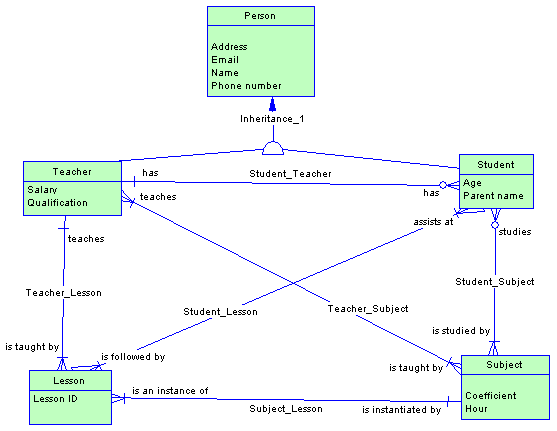
\includegraphics[width=10cm]{../img/Conceptual_Model_PowerDesigner}
	\caption{\TODO{Conceptual diagram}\cite{ConceptualModelExample}}
\end{figure}

\subsection{Logical Data Model}

Keeping its structure generic a logical model extends the objects described in a conceptual data model making it not that easy to read but becomes a good base documentation for an implementation. Data requirements are described from business point of view.

\subsubsection{Characteristics}
\begin{itemize}
	\item Independent of a software used to manage the data or DBMS.
	\item Each entity has the primary key.
	\item Foreign keys are expressed.
	\item Data types description is introduced (but in a way that is not tied with any specific technology).
	\item Normalized up to \TODO{third normal form}.
\end{itemize}
\definition{Entities}, \definition{attributes} and \definition{relationships} from a conceptual model are present on this layer as well. Relationships are not that abstract as before and keys that actually make relationship happen between entities are added as their attributes.

\begin{figure}[H]
	\centering
	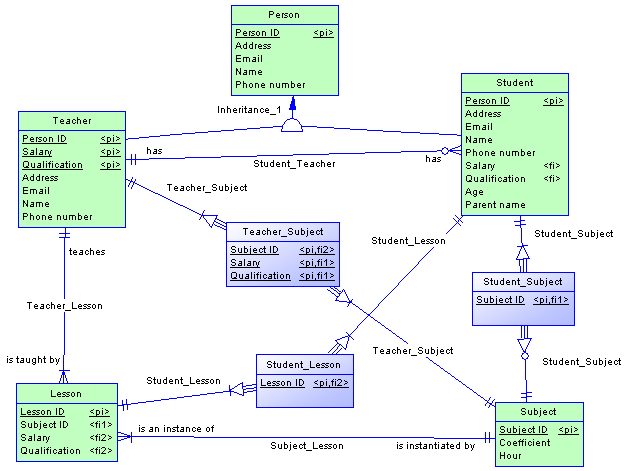
\includegraphics[width=10cm]{../img/Logical_Model_PowerDesigner}
	\caption{\TODO{Logical diagram}\cite{LogicalModelExample}}
\end{figure}

\subsection{Physical Data Model}

A physical data is a description of a database implementation so it is necessarily tied with one specific database technology as it should have one-to-one mapping to actual implementation. Its main message is to communicate how the data are stored.

\subsubsection{Characteristics}
\begin{itemize}
	\item Exact data types (DBMS specific) and default values of columns are outlined.
	\item DBMS's naming conventions are applied on objects.
	\item Constraints are defined (eg. not null, keys, or unique for columns).
	\item Contains validation rules, database triggers, indexes, stored procedures, domains, and access constraints.
	\item Normalization in order to avoid data redundancy or de-normalized if performance increase is reflected in the model.
\end{itemize}

Objects in physical models should reflect database organization and at the same moment related higher-level concepts should be transformable to physical level. \definition{Tables} should store records that corresponds to logical entities and \definition{columns} represent previously described attributes in memory.
Commonly schemas\footnote{Plural of the word schema is schemata but in literature about database design the word schemas is used} are present. A \definition{schema} is basically container for tables that logically groups them. Users have usually schemas assigned and can access only the tables contained in those schemas.

\begin{figure}[H]
	\centering
	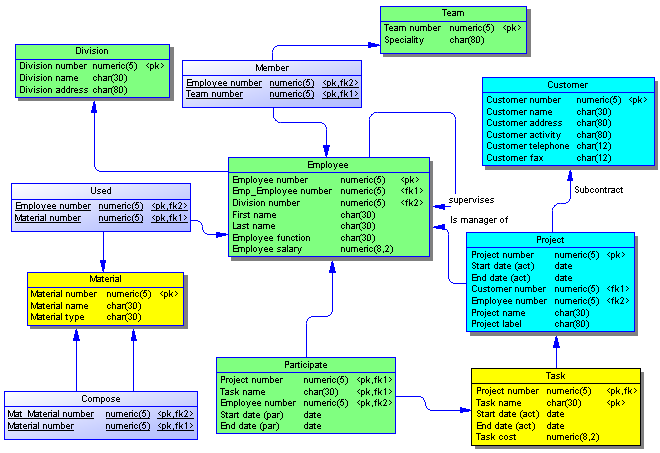
\includegraphics[width=10cm]{../img/Physical_Model_PowerDesigner}
	\caption{\TODO{Physical diagram}\cite{PhysicalModelExample}}
\end{figure}

\section{Relations Between the Models}

We described what the role of each of the layers in a database design process is.
Now we will show that the data models are somehow connected vertically and what are the implications.

When talking about vertical divisions, we should think about how database design can proceed.

The basic approach is the \definition{top-down approach} to database modeling.
It is natural to start with a general idea what should a database store and what are the relations between stored object. 
End-user defines this high-level logic and as time goes importance of a database designer grows until he is at full charge and develops a complete database. It is the most common case of database development when a client identifies a high-level need for a database and hires an expert in this domain to make it happen.

The other way to create full view of a database is the \definition{bottom-up approach}. It can be harder to imagine what would be use-cases for this approach, but there are some problems that are bottom-up in nature. A nice real world example of bottom-up strategy is how doctors work. 
They start with "low-level" details such as symptoms and they're trying to build the whole image of patient's condition. So in the field of software data elements are firstly identified and after they are logically grouped to form bigger units, entities, and so on until the full hierarchy is known.

\subsection{Maps-to Relation}

In order to capture how high-level concepts are actually realized by more precise object a relation that we will call \definition{maps-to} is used. The relation leads between objects that are semantically equivalent on different levels of abstraction, sometimes even mapping between objects on the same layer are allowed but we will not consider this, as we consider it be mixing two different concepts together - data modeling with data lineage. To be more precise what we mean by semantically equivalent objects in data models is that we will assume maps-to edges solely source is model and target is model, entity and table, attribute and column, or the other way around.
Following these mapping links is extremely useful when a person wants to gain an overall overview of the system and comprehend it. For example when a user sees a data table in physical model that has a technical name that obey some naming convention and due to normalization does not represent any object straightforwardly, he can follow mapping links that leads to higher layer providing greater  abstraction over the implementation and the motivation why the table was created should be much clearer then.
It is worth mentioning that usually the mapping relations between objects of different layers simple one-to-one relationships but the cardinalities may vary greatly. For example one logical attribute may be realized via multiple database columns.
Normally more technical models are composed of bigger count of objects so one conceptual entity may be realized by multiple database tables in the end. Generally it is assumed that number of conceptual objects $<$ number of logical objects $<$ number of physical objects. It is natural that when capturing important high-level aims less entities is needed to express the intention but as we are getting closer to the implementation more necessary details come to play.

